\documentclass{beamer}
\usepackage[utf8]{inputenc}
\usepackage{hyperref}

\usepackage{tikz}

\usepackage{latexsym,xcolor,multicol,booktabs,calligra}
\usepackage{amsmath,amssymb,BOONDOX-cal,bm}	
\usepackage{graphicx,pstricks,stackengine} 
\usepackage{libertinus}
\usepackage{amssymb}
\usepackage{pgfplots}
\usepackage{tikz}
\usepackage{xcolor}
\usetikzlibrary{positioning}




\usepackage{etoolbox}
\makeatletter
\newcommand{\noframenumbering}{%
  \beamer@noframenumberingtrue%
}
\makeatother

\usepackage[T1]{fontenc}

\usepackage{hyperref}
\hypersetup{
    colorlinks=true,
    linkcolor=blue,
    urlcolor=blue,
    citecolor=blue
}

\title{Macroeconometrics\\
6 - Beyond Linearity: Thresholds, Asymmetries, Regime Changes (TVAR, ST-VAR, Markov switching, TVP-VAR\& Local Projections)}
\author{Camille Souffron\\
Ecole Normale Supérieure \& Paris School of Economics\\
\textcolor{blue}{\href{mailto:camille.souffron@ens.psl.eu}{camille.souffron@ens.psl.eu}}}
\institute{\normalsize M2 EPOG JM}
\date{Fall 2026}

\usetheme{Singapore}

\def\cmd#1{\texttt{\color{red}\footnotesize $\backslash$#1}}
\def\env#1{\texttt{\color{RoyalBlue}\footnotesize #1}}

\newtheorem{thm}{Theorem}[theorem]
\setbeamertemplate{footline}[frame number]

\begin{document}

\begin{frame} % <-- no [plain] here!
    \titlepage % This keeps the theme style
    \begin{center}
        
\includegraphics[width=0.4\textwidth]{logos.png}
    \end{center}
\end{frame}



\addtocounter{framenumber}{-1}





%======================================================
\begin{frame}{A note on Proxy-VARs (SVARs with External Instruments)}
%======================================================
\scriptsize

\begin{itemize}
  \item Narrative shocks and high-frequency surprises are \emph{noisy measures} of a true structural shock.
  \item If put directly in the VAR, noise $\Rightarrow$ attenuation bias and misspecified dynamics.
  \item Proxy-VARs treat the series as an \emph{external instrument} (i.e. using its covariance with VAR residuals)
\end{itemize}

\textbf{Setup:} Observed proxy $z_t$ is $z_t = \lambda\,\varepsilon_t^{*} + \eta_t$ i.e. a noisy signal of the target shock $\varepsilon_t^{*}$, uncorrelated with all other shocks.

\textbf{Instrument validity conditions}
\begin{itemize}
  \item \textbf{Relevance:} $\mathrm{Cov}(z_t,\varepsilon_t^{*}) \neq 0$ (proxy contains signal).
  \item \textbf{Exogeneity:} $\mathrm{Cov}(z_t,\varepsilon_t^{j}) = 0$ for $j\neq *$ (noise is orthogonal to other shocks).
\end{itemize}

\textbf{How (Proxy-SVAR)}
\begin{enumerate}
  \item Estimate reduced-form VAR $\Rightarrow$ obtain residuals $u_t$.
  \item Identify impact vector of the target shock:
  \[
      b_* \propto \mathbb{E}[u_t\, z_t] \text{ the covariance vector}
  \]
  because only the column of $B$ associated with $\varepsilon_t^{*}$ covaries with $z_t$.
  \item Normalize $b_*$ to a 1-unit shock and compute IRFs as usual.
\end{enumerate}

\textbf{Alternative (LP-IV)}
\begin{itemize}
  \item For each horizon $h$: regress $y_{t+h}$ on $u_t$ and lags, instrument $u_t$ with $z_t$.
  \item The IV coefficient $\theta_h$ is the IRF at horizon $h$.
\end{itemize}

Check first-stage strength (F-stat) to avoid weak instrument bias, use robust inference (HAC/Bootstrap), and verify economic sign/shape.
\end{frame}




\section{Introduction}

\begin{frame}{WHAT THE HECK ARE SHOCKS?}
\footnotesize

\pause

\footnotesize

More on this during classes on structural modelling, but a \textbf{critical issue} in \textit{mainstream} modelling!

\medskip

DSGEs need to assume (a LOT of) shocks to be identified (otherwise, \textit{stochastic singularity}).

\medskip

Real \textit{ontological} shocks (exogenous causes)? Or just th\textbf{e \textit{measure of our ignorance}?} (same question for the so-called "Solow's residual" - actually change in labour hoarding, in capacity utilization, in capital vintages etc)

\medskip

Shocks, or\textit{\textbf{ endogenous fluctuations from nonlinear dynamics}} thus not recognized by those linear specifications? 

\begin{figure}
    \centering
    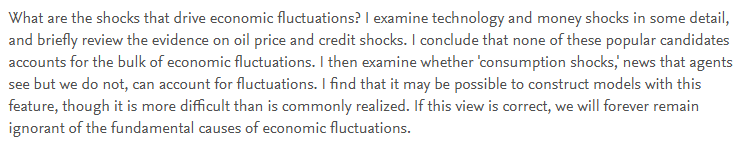
\includegraphics[width=1.1\linewidth]{Cochrane abstract.png}
    \caption{\footnotesize Abstract of "Shocks", John Cochrane (1994), NBER WP.}
\end{figure}

\end{frame}




\begin{frame}{WHAT THE HECK ARE SHOCKS?}

Remember that the "well-lag-specified" condition is that \textbf{there is enough lags for the residual to be a white noise. }

\medskip
But it does\textbf{ not }mean than in the social realm, it happens \textit{ex nihilo}.

\medskip
It means that \textbf{we've extracted in a LINEAR way all the useful information from the past.} But the specification is "only" a linear one (linear regressions, i.e. controlled correlations). The residual is thus, \textbf{"conditionally on past variables and available data, linearly unpredictable".}

\medskip
It can for example be the fruit of a nonlinear element that is NOT captured by the linear specification (whatever the number of lags). 
\end{frame}


\begin{frame}{Impulse Response Functions (IRF) - Linearity}
\textbf{LIMITS OF LINEARITY}
\scriptsize
\smallskip
\begin{itemize}
    \item \textbf{As VARs are linear, a positive shock is the mirror image of a negative shock. }Only non-linear models can account for asymmetry.
    \begin{itemize}
    \scriptsize
        \item Always true in reality? \pause
        \item  Have the macro multipliers the same magnitude during expansion and during recession? E.g. Greek crisis (LMAO). And not only: multipliers may be higher at the ZLB (Christiano et al., 2011).
    \end{itemize}
    \item \textbf{As VARs are linear, the magnitude of the initial shock doesn’t matter in constructing the IRF.}
    \begin{itemize}
    \scriptsize
        \item Usually, a "unit shock" is a \textbf{one-standard-deviation shock} to the residual of a variable.
        \item 2.3 unit shock $\Longrightarrow$ 2.3 impulse response. 
        \item Always true in reality? \pause
        \item Thresholds? Tipping points? (e.g. the \textit{Great Moderation}, key rates and Minskyan moment). 
    \end{itemize}
     \pause
    \item \textbf{Stable linear VARs always converge to a unique equilibrium.}
    \begin{itemize}
    \scriptsize
        \item A stable VAR$(p)$ has MA($\infty$) form $y_t = \sum_{h=0}^{\infty} \Phi_h u_{t-h},\qquad \Phi_h \to 0 \text{ if stable}$
    \begin{itemize}
    \scriptsize
\item Hence if $\Phi_h \to 0$ (all eigenvalues $<1$):
    \end{itemize}
\[
\mathbb{E}[y_{t+h}\mid y_t] \to 0 \quad
(\text{or }\mu \text{ if not demeaned}).
 \]
        \item \textbf{Unstable linear VAR} ($|\lambda|\ge1$): $\Phi_h$ does not shrink → forecasts \textbf{explode}.
    \end{itemize}
\end{itemize}

\end{frame}






%======================================================
\begin{frame}{}
%======================================================
\small

\begin{itemize}
  \item The \textbf{impulse responses are time invariant} (applies
        \emph{everywhere and always})
        \[
          \text{IRF}_h = \frac{\partial y_{t+h}}{\partial \varepsilon_t},
          \quad \text{independent of the state of the economy.}
        \]
  \item Same shock $\varepsilon_t$ $\Rightarrow$ same response, whether we are
        in a boom or in a recession, with low or high leverage, at the ZLB or not.
\end{itemize}

\pause
\textbf{But macro facts are strongly state-dependent:}
\begin{itemize}
  \item \textbf{Asymmetry of cycles:} recessions are sharp and deep,
        expansions slow and mild.
        \begin{itemize}
          \item Linear SVAR $\Rightarrow$ symmetric responses to positive vs negative shocks.
        \end{itemize}
  \item \textbf{ZLB / policy nonlinearity:} the central bank reacts very
        differently when the policy rate is near zero.
  \item \textbf{Tipping points and financial crises:} a leverage shock in
        "normal" times is not the same as the \emph{same} shock in an already
        fragile, highly-leveraged system.
\end{itemize}

\begin{itemize}
  \item Nonlinear models allow \textbf{state-dependent IRFs}
\end{itemize}

\end{frame}





%======================================================
\begin{frame}{Uncorrelated vs.\ Independent Shocks}
%======================================================
\footnotesize
At the core of \textbf{linear} TS: after enough lags, the residual is assumed to be \textbf{white noise} ($\mathbb{E}[u_t]=0, \qquad \text{Cov}(u_t,u_{t-h})=0 \ \forall h\neq 0$), i.e.
 \[
    \Rightarrow u_t \text{ is \emph{linearly} unpredictable from the past.}
  \]
But does \textbf{uncorrelated $\Rightarrow$ independent? }\pause NOT IN GENERAL! There can still be \textbf{nonlinear dependence!} (correlation is linear) 
\medskip

\textbf{Special case: Gaussian shocks}. If $\{u_t\}$ is a \textbf{jointly Gaussian process} and
        $\text{Cov}(u_t,u_{t-h})=0$ for all $h\neq 0$, then:
\[
          (u_t, u_{t-1}, u_{t-2},\dots) \text{ is multivariate normal with diagonal covariance.}
        \]
        For a multivariate normal, \textbf{zero covariance $\Rightarrow$ independence} (= \textit{Gaussian} white noise)
        Linearly unpredictable = \textbf{fully unpredictable}.

\pause
\medskip
\textbf{In macro/finance reality:}
\begin{itemize}
  \item Residuals often look uncorrelated, but they are \textbf{not} jointly Gaussian:
  \item There is no remaining structure in the full conditional distribution of \( y_t \mid \mathcal{X}_{t-1} \).
Two big ways extra structure can hide:
\begin{itemize}
\footnotesize
    \item \textbf{Nonlinear conditional mean} (TAR / STAR / MS-VAR / TVP).
    \item \textbf{Nonlinear conditional variance or higher moments} (ARCH / GARCH / SV).
\end{itemize}
\end{itemize}
\textbf{$=$ Motivation for nonlinear TS models!}
\end{frame}





















\section{Nonlin}

%======================================================
\begin{frame}{What does "nonlinear" actually mean here?}
%======================================================
\small

\textbf{Question:} in time-series / macro, \emph{where} can nonlinearity enter?

\medskip
\pause
\textbf{1. Nonlinear in levels (functional form)}
\begin{itemize}

  \item Example (powered regressors, logs, interactions, saturating functions):
\[
    y_t = \alpha
          + \beta_1 x_t + \beta_2 x_t^2
          + \beta_3 \log x_t
          + \beta_4 (1 - e^{-\lambda x_t})
          + \beta_5 \frac{x_t}{1+\gamma x_t}
          + \beta_6 (x_t \cdot z_t)
          + u_t
  \]

  \item These are \textbf{nonlinear transformations of regressors}, but the model
        remains \textbf{linear in the parameters} $(\alpha,\beta_1,\dots)$ (with $\lambda$ and $\gamma$ calibrated) $\Rightarrow$ OLS is still valid (\textbf{H1}).
        \begin{itemize}
            \item OLS simply treats $x_t^2$, $\log x_t$, $(1-e^{-\lambda x_t})$,  or $\tfrac{x_t}{1+\gamma x_t}$ as additional regressors.
        \end{itemize}

  \item Very common in cross-section / panel.  
        In time series, usually a \textbf{mild / static} form of nonlinearity
        (it does not change the dynamics of the system).

\end{itemize}

\end{frame}


%======================================================
\begin{frame}{Can we approximate nonlinear DGPs with powers?}
%======================================================
\footnotesize

\textbf{Yes.}  
If the true DGP is 
\[
y_i = f(x_i) + u_i,
\]
with $f$ continuous, then by the \textbf{Weierstrass approximation theorem}:
\[
f(x) \approx \beta_0 + \beta_1 x + \beta_2 x^2 + \dots + \beta_p x^p
\quad \text{for $p$ large enough.}
\]

\begin{itemize}
  \item This preserves \textbf{linearity in parameters} $\Rightarrow$ OLS satisfies H1.
  \item OLS simply treats $x, x^2, \dots, x^p$ as additional regressors.
\end{itemize}

\pause
\textbf{But in practice, polynomial approximation is often risky:}
\begin{itemize}
  \item \textbf{Boundary explosions:} high-degree polynomials oscillate and extrapolate poorly.
  \item \textbf{Multicollinearity:} $x, x^2, x^3,\dots$ highly correlated $\Rightarrow$ large standard errors.
  \item \textbf{Overfitting:} large $p$ fits noise rather than signal.
  \item \textbf{Poor global fit} for S-shaped / saturating patterns (logistic, $1-e^{-\lambda x}$, $\frac{x}{1+\gamma x}$), and you put functional parameter $\lambda$ exogenously!
\end{itemize}

\textbf{Hence in applied work:} low-degree polynomials (quadratic, cubic) are fine, but rich nonlinearities are better captured with \textbf{splines}.


\end{frame}


%======================================================
\begin{frame}{What does "nonlinear" actually mean here?}
%======================================================
\small

\textbf{2. Nonlinear dynamics (what matters for cycles)}
\begin{itemize}
  \item \textbf{Threshold / piecewise linear:} dynamics change when a state variable
        crosses a threshold (e.g. recession vs expansion).
  \item \textbf{Smooth transition:} coefficients change \emph{gradually} with a
        state variable (e.g. output gap, credit-to-GDP).
  \item \textbf{Regime-switching:} coefficients depend on a (possibly latent)
        regime index $s_t$ (e.g. "crisis" vs "normal" times).
  \item \textbf{Time-varying parameters:} coefficients drift over time
        (policy learning, structural change, financial development).
\end{itemize}

\bigskip
\pause
\textbf{3. Nonlinear in shocks (error process)}
\begin{itemize}
  \item The \textbf{variance} of shocks can depend on the past or on the state:
        \emph{conditional heteroskedasticity}.
  \item \textbf{ARCH/GARCH models:} volatility of $u_t$ increases when past shocks
        were large - capture volatility clustering and "turbulent" periods.
  \item We \textbf{won't study ARCH/GARCH in this class}, but show that
        even with \emph{linear} conditional mean, risk dynamics can be highly nonlinear.
\end{itemize}

\end{frame}



%======================================================
\begin{frame}{}
%======================================================
\footnotesize

\begin{table}[h!]
\centering
\begin{tabular}{p{0.26\textwidth} p{0.18\textwidth} p{0.20\textwidth} p{0.28\textwidth}}
\toprule
\textbf{Model} &
\textbf{Abrupt vs.\ Smooth} &
\textbf{State variable} &
\textbf{State evolution} \\
\midrule

(1) Threshold / Piecewise linear
& Abrupt jump
& Observed
& Deterministic rule ($z_t > c$) \\[0.4em]

(2) Smooth transition (STAR / STVAR)
& Smooth change
& Observed
& Smooth deterministic function of $z_t$ \\[0.4em]

(3) Regime switching (MS-VAR)
& Abrupt jump
& Latent $s_t$ (must infer it from the data)
& Probabilistic Markov chain \\[0.4em]

(4) Time-varying parameters (TVP-VAR)
& Smooth drift
& Latent parameters (must infer it from the data)
& Slow stochastic drift (random walk) \\
\bottomrule
\end{tabular}
\end{table}

\textbf{Observed vs.\ latent state, and abrupt vs.\ smooth evolution}
\end{frame}



\section{TAR}

%======================================================
\begin{frame}{Threshold autoregression (TAR): univariate}
%======================================================
\small
Introduced by Tong (1978) and Tong \& Lim (1980).
Simplest case: one variable, two regimes. \textbf{Threshold AR(1):}

\[
y_t =
\begin{cases}
\phi_1 y_{t-1} + u_t, & \text{if } z_{t-d} \le c \quad (\text{Regime 1}) \\
\phi_2 y_{t-1} + u_t, & \text{if } z_{t-d} > c \quad (\text{Regime 2})
\end{cases}
\]

\begin{itemize}
  \item $z_{t-d}$: \textbf{threshold variable} (e.g.\ output gap, credit, unemployment),
        possibly lagged by $d$ periods.
  \item $c$: \textbf{threshold level}.
  \item If $\forall t,\ z_t = x_t$, the process is called a \emph{self-exciting TAR} (SETAR) process.
\end{itemize}

\begin{itemize}
  \item In each regime, dynamics are \emph{linear AR(1)}, but globally, the process is \textbf{nonlinear}, because the coefficient\textbf{ switches} when $z_{t-d}$ crosses $c$.
\end{itemize}

\textbf{Indicator-function representation:}
\[
I_t = \mathbf{1}\{z_{t-d} > c\}, \qquad
y_t = \big(\phi_1 + (\phi_2 - \phi_1) I_t \big) y_{t-1} + u_t
\]
Coefficient on $y_{t-1}$ depends on the \textbf{state} $I_t$ (indicator-function: takes $1$ if $z_{t-d} > c$, $0$ otherwise).

\end{frame}

%======================================================
\begin{frame}{TAR dynamics: interpretation}
%======================================================
\small

\textbf{Regime-specific persistence:}
\begin{itemize}
  \item If $|\phi_1| < |\phi_2|$, then $y_t$ is more \textbf{persistent} in Regime 2
        than in Regime 1 (or vice versa).
        \item $\Longrightarrow$ \textbf{state-dependent speed of adjustment}.
\end{itemize}

\begin{itemize}
  \item The economy may behave differently in \textbf{recessions} than in
        \textbf{booms}:
        \begin{itemize}
          \item fast mean reversion when output is far below trend;
          \item slower mean reversion when near or above trend.
        \end{itemize}
  \item Example: let $z_{t-d}$ be the output gap. For $z_{t-d} \ll 0$,
        policy reaction and private behaviour may change.
\end{itemize}

\textbf{Stationarity:}
\begin{itemize}
  \item Each regime separately: behaves like an AR(1); if $|\phi_1|<1$ and $|\phi_2|<1$,
        the process tends to revert in both regimes.

\end{itemize}



\end{frame}

%======================================================
\begin{frame}{Threshold VAR (TVAR)}
%======================================================
\small

\textbf{From univariate TAR to multivariate VAR:}

Let $y_t$ be a $k \times 1$ vector and consider a VAR($p$) with two regimes:

\[
y_t =
\begin{cases}
A_0^{(L)} + A_1^{(L)} y_{t-1} + \dots + A_p^{(L)} y_{t-p} + u_t,
& \text{if } z_{t-d} \le c \quad (\text{Low state})\\[0.2cm]
A_0^{(H)} + A_1^{(H)} y_{t-1} + \dots + A_p^{(H)} y_{t-p} + u_t,
& \text{if } z_{t-d} > c \quad (\text{High state})
\end{cases}
\]

\begin{itemize}
  \item $A_j^{(L)}, A_j^{(H)}$ are $k \times k$ coefficient matrices in each regime.
  \item The\textbf{ threshold variable} $z_{t-d}$ can be \textbf{one component of }$y_{t-d}$ (e.g.\ credit),
        or some\textbf{ external macro-financial indicator.}
\end{itemize}

\textbf{Indicator representation:}
\[
I_t = \mathbf{1}\{z_{t-d} > c\}, \quad
y_t = A_0(I_t) + \sum_{j=1}^p A_j(I_t)\, y_{t-j} + u_t,
\]
where
\[
A_j(I_t) = A_j^{(L)} + \big(A_j^{(H)} - A_j^{(L)}\big) I_t
\]

\begin{itemize}
  \item Globally, the model is nonlinear because coefficients switch with $I_t$.
\end{itemize}

\end{frame}


%======================================================
\begin{frame}{Allows for regime-specific intercepts}
%======================================================
\small

\textbf{Intercepts can also switch across regimes (not only slopes/persistence).}

\[
y_t =
\begin{cases}
\mu_1 + \phi_1 y_{t-1} + u_t, & z_{t-d} \le c \\[0.2em]
\mu_2 + \phi_2 y_{t-1} + u_t, & z_{t-d} > c
\end{cases}
\]

\begin{itemize}
  \item $\mu_1 \neq \mu_2$ captures \textbf{state-dependent means} /
        \textbf{level shifts} across regimes.
  \item Useful when the economy displays different average levels.
\end{itemize}

\medskip

\textbf{More than two regimes?}
\begin{itemize}
  \item TAR/TVAR models can be generalised to \textbf{3 or more regimes! (e.g. expansion vs recession... vs normal time?)}
  \item But grid search over multiple thresholds becomes computationally very demanding (search space explodes).
  \item \textbf{Gonzalo \& Pitarakis (2002)} propose a sequential procedure to select the number of regimes efficiently.
\end{itemize}

\end{frame}


%======================================================
\begin{frame}{TVAR: state-dependent IRF}
%======================================================
\small

\textbf{Within each regime:} we have an ordinary linear VAR.

\begin{itemize}
  \item In the low state ($z_{t-d} \le c$), dynamics are governed by
        $\{A_j^{(L)}\}_{j=1}^p$
  \item In the high state ($z_{t-d} > c$), dynamics are governed by
        $\{A_j^{(H)}\}_{j=1}^p$
\end{itemize}

\textbf{State-dependent IRFs:} In each regime, we can use the usual VAR machinery
        (companion form, powers of the transition matrix) to compute IRFs.
\[
\text{IRF}_h^{(L)} =
\frac{\partial y_{t+h}}{\partial \varepsilon_t} \Big|_{z_{t-d} \le c}
\qquad
\text{IRF}_h^{(H)} =
\frac{\partial y_{t+h}}{\partial \varepsilon_t} \Big|_{z_{t-d} > c}
\]

\begin{itemize}
  \item The same shock can have different effects
        depending on whether the economy is in a “normal” or “stressed” state.
  \item \textbf{Identification:} within each regime, we can still apply
        standard schemes to recover \textbf{structural shocks} ($\varepsilon_t = C^{-1}u_t$, e.g.\ Cholesky).
  \item Here we implicitly consider \textbf{fixed-state IRFs}: we study the response as if the economy stayed in the given regime over the horizon.\textbf{ So need realistic horizon! (a.g. avoid assuming a recession $>$ 5y if no empirical basis)}
\end{itemize}

\end{frame}


%======================================================
\begin{frame}{Estimating \& Testing a TVAR}
%======================================================
\scriptsize

\textbf{Goal:} estimate $\{A_j^{(L)}, A_j^{(H)}\}$, the threshold $c$, and (optionally) the delay $d$.

\medskip
\textbf{Simplest approach: grid search over $c$.}
\begin{enumerate}
  \item Choose a grid of candidate thresholds $c \in \mathcal{C}$
        (e.g.\ between lower and upper quantiles of $z_{t-d}$, trimming extremes).
  \item For each $c \in \mathcal{C}$:
        \begin{itemize}
        \scriptsize
          \item split the sample into two subsamples:
                $\{t : z_{t-d} \le c\}$ and $\{t : z_{t-d} > c\}$;
          \item estimate two separate VAR($p$)s by OLS; compute the sum of squared residuals
                $\text{SSR}(c)$.
        \end{itemize}
  \item Select $\hat{c}$ that minimises $\text{SSR}(c)$.
\end{enumerate}

\begin{itemize}
  \item Called \textbf{Sequential Conditional Least Squares}. 
\item NB: under Gaussian shocks, LS coincides with \textbf{MLE}.
  \item In practice we also search over delay $d$ and lag orders $(p_1,p_2)$ and pick the combination that minimises an information criterion (AIC/BIC) over $(c,d,p_1,p_2)$.
\end{itemize}

\medskip
\textbf{Testing linear VAR vs TVAR:}
\begin{itemize}
  \item Null hypothesis: \textbf{no threshold}, i.e.\ $A_j^{(L)} = A_j^{(H)}$ for all $j$.
  \item Under $H_0$, the model collapses to a \emph{single} VAR, so the threshold
        $c$ becomes \textbf{irrelevant and thus not identified} (every $c$ works UNDER $H_0$, same model)! 
        \item Because $c$ is only defined under the alternative, usual Wald/F-tests
        have \textbf{nonstandard} distributions (cannot use standard critical values).
  \item Solution: \textbf{sup-Wald} tests with \textbf{bootstrap} critical values
        (we do not derive them here, but it is important to know why they are needed).
\end{itemize}

\end{frame}



 \section{STAR \& GIRFs}
 
%======================================================
\begin{frame}{Smooth transition (STAR)}
%======================================================
\footnotesize

\textbf{Issue with hard thresholds} is that regime switches can be unrealistically
\emph{abrupt} at $z_{t-d} = c$.

\medskip
\textbf{Smooth Transition AR (STAR)} (Ter\`{a}svirta \& Anderson, 1992; Granger \& Ter\`{a}svirta, 1993; Ter\`{a}svirta, 1994):
\[
y_t = \big( \phi_1 + (\phi_2 - \phi_1) G(z_{t-d}) \big) y_{t-1} + u_t
\]
where $G(\cdot)$ is a \textbf{smooth }function, typically\textbf{ logistic}:
\[
G(z_{t-d}) = 
\frac{1}{1 + \exp\{-\gamma (z_{t-d} - c)\}},
\quad \gamma > 0
\]

\begin{itemize}
  \item $G(z_{t-d}) \in (0,1)$ is a \textbf{transition function}.
  \item For $z_{t-d} \ll c$ (far below threshold): $G \approx 0$, coefficient $\approx \phi_1$.
  \item For $z_{t-d} \gg c$ (far above threshold): $G \approx 1$, coefficient $\approx \phi_2$.
  \item   In between, coefficients are a \textbf{smooth mixture} of $\phi_1$ and $\phi_2$.
  \item Parameter $\gamma$ controls how \textbf{fast} we move from Regime 1 to Regime 2.
\end{itemize}

\begin{itemize}
  \item \textbf{STAR: gradual change as $z_{t-d}$ approaches and crosses $c$.}
  \item As $\gamma \to \infty$, $G(z_{t-d})$ approximates the hard indicator (TAR): abrupt switching (STAR $\to$ TAR).
\end{itemize}

\end{frame}



\begin{frame}{Examples of logistic function for various $\gamma$}
\begin{figure}
    \centering
    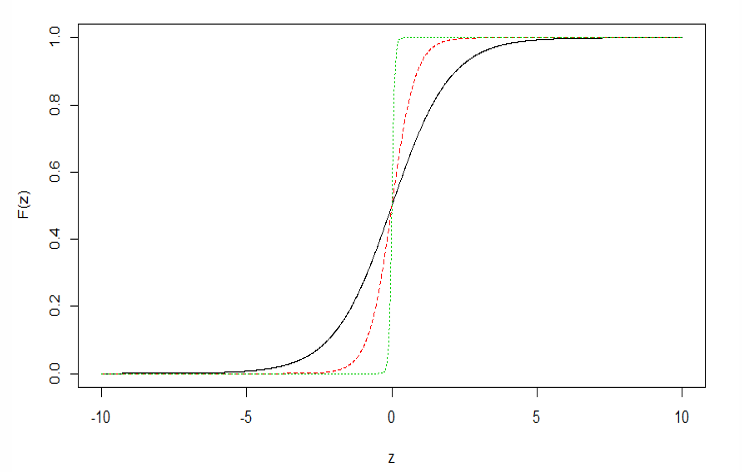
\includegraphics[width=1\linewidth]{logistic 1.png}
\end{figure}
    
\end{frame}
%======================================================
\begin{frame}{Estimating and testing a ST-VAR}
%======================================================
\footnotesize

\textbf{Estimation:}
\begin{itemize}
  \item Estimate $(A_j^{(L)}, A_j^{(H)}, c, \gamma)$ by
        \textbf{Nonlinear Least Squares} (i.e. minimise the sum of squared residuals
        $\sum_t \|y_t - H(y_{t-1},\dots;\theta)\|^2$).
  \item Again, if the innovations are Gaussian, NLS coincides with \textbf{(quasi-)maximum likelihood} and is consistent / asymptotically normal under standard regularity conditions.
  \item Conceptually: still two linear VARs, \textbf{smoothly glued} together
        by the transition function $G(z_{t-d};c,\gamma)$.
\end{itemize}

\textbf{Testing linear VAR vs STVAR:}
\begin{itemize}
  \item $H_0$: \textbf{linearity} (no smooth transition), i.e.\ $A_j^{(L)} = A_j^{(H)}$.
  \item Still same issue under $H_0$ of linearity: the transition parameters $(c,\gamma)$ are
        \textbf{not identified} $\Rightarrow$ naive Wald tests are invalid.
  \item Solution (Luukkonen-Saikkonen-Teräsvirta): use an \textbf{auxiliary
        regression} (Taylor expansion of $G$ around $\gamma=0$) and test
        linearity with a standard $F$/$\chi^2$ test.
\end{itemize}


\end{frame}

%======================================================
\begin{frame}{ST-VAR: state-dependent but smooth IRFs}
%======================================================
\small
\textbf{Smooth transition extension of TVAR:} the VAR becomes
\[
y_t = A_0(z_{t-d}) + \sum_{j=1}^p A_j(z_{t-d})\, y_{t-j} + u_t
\]
with $
A_j(z_{t-d}) = A_j^{(L)} + \big(A_j^{(H)} - A_j^{(L)}\big) G(z_{t-d}), \quad j=0,\dots,p.$ In between, the effective coefficients are a \textbf{smooth mixture} of $A_j^{(L)}$ and $A_j^{(H)}$.

\textbf{IRFs now depend continuously on a MIXTURE $G$ of states since it is smooth:} $  \text{IRF}_h\big(z_{t-d}\big) =
        \frac{\partial y_{t+h}}{\partial \varepsilon_t}
        \Big|_{z_{t-d}}$. We decide for the value of $z_{t-d}$.

NB: "only" state-dependent IRF, i.e.t IRF when $t=2008recession$ will be the same as IRF when $t=1991recession)$.
\medskip

Actually, is it realistic to consider an impact in recession at $t=0$ without ever returning to expansion? 
\end{frame}




%======================================================
\begin{frame}{IRFs in nonlinear VARs: fixed vs dynamic state}
%======================================================
\scriptsize

\textbf{In TVAR/ST-VAR models, impulse responses are no longer unique: they depend on the \emph{state} (transition variable $z_{t-d}$).} \textbf{Three concepts to distinguish:}

\medskip

\textbf{1. Fixed-state IRF with exogenous $z_t$ (outside the VAR)}
  \begin{itemize}
    \item We fix $z_{t-d}=z^\ast$ and keep it constant over the horizon. IRFs are then those of a \textbf{linear VAR} with coefficients $A_j^{\text{eff}}(z^\ast)$: clear interpretation as IRF in regime $z^\ast$.
  \end{itemize}

\textbf{2. Fixed-state IRF with \emph{endogenous} $z_t$}
  \begin{itemize}
    \item Now $z_t$ is one component of $y_t$, and thus reacts to shocks.
    \item Standard state-dependent IRFs often proceed by fixing $z_{t-d}=z^\ast$ \emph{and holding it fixed over $h$},
    implicitly freezing $G$. $\Rightarrow$ \textbf{Local IRF} conditional on being in state $z^\ast$ at $t$, but \textbf{counterfactual} for longer horizons.
    \end{itemize}
    
\textbf{Problems:}
\begin{enumerate}
    \item Even if the shock occurs in state 1, the economy may gradually change state while it still has an effect (i.e. at relevant horizon).
    \item Counterfactually, the shock itself may cause a change of state (i.e. impact the transition variable)! Missed by the forcing to maintain a constant state.
    \item Conversely, the shock may amplify the state even without the assumption of a constant state, which would have been missed under the latter assumption.
\end{enumerate}
\end{frame}



%======================================================
\begin{frame}{IRFs in nonlinear models: Generalized IRFs (GIRFs)}
%======================================================
\scriptsize
\textbf{3. Dynamic-state (or path-dependent) IRF with endogenous $z_t$}
  \begin{itemize}
    \item Start from a given initial state/history, let the shock hit at $t$, and then let $z_{t+h}$ and $G_{t+h}$ \textbf{evolve endogenously} according to the estimated nonlinear model. Allows for regime changes.
    \item This delivers a genuinely \textbf{state-dependent, path-dependent IRF}:
    \[
      IRF_h\big(z_{t-d}, \varepsilon_t\big) = \frac{\partial y_{t+h}}{\partial \varepsilon_t}
      \Big|_{\text{state and path implied by the model}}
    \]
    \item However, this is still a \textbf{single-path} IRF: no averaging over future shocks yet.
  \end{itemize}

\textbf{4. Generalized IRF (GIRF, Koop-Pesaran-Potter, 1996):}
\textbf{Goal:} capture the effect of a shock when
\begin{itemize}
  \item future states (regimes) and transition variables $z_t$ evolve \textbf{endogenously},
  \item and future innovations are \textbf{random}.
\end{itemize}

\medskip

\[
  \mathrm{GIRF}_h(x_{t-1}, \delta)
  = \mathbb{E}\big[y_{t+h} \mid \varepsilon_t = \delta,\, x_{t-1}\big]
    - \mathbb{E}\big[y_{t+h} \mid x_{t-1}\big],
\]
where
\begin{itemize}
  \item Condition on a \textbf{given starting state} $x_{t-1}$ then \textbf{average over future shocks \emph{and} future regimes}  (because things happen after $t_0=1997$).
  \item In practice: simulate many paths with/without the shock $\varepsilon_t=\delta$ (Monte Carlo), from chosen histories, and average the difference.
        \item Allow for conditional IRF at $t=0$ but then\textbf{ unconditional} along the horizon. I.e. \textbf{future regimes and transition variables evolve \emph{endogenously} }, integrating uncertainty. 

\end{itemize}

\end{frame}



%======================================================
\begin{frame}{An example of ST-VAR application}
%======================================================
\small

\textbf{Reference:}
Caggiano, Castelnuovo \& Groshenny (2014),
\emph{``Uncertainty shocks and unemployment dynamics in U.S. recessions''}, JME.

\medskip

\textbf{Main question:}
\begin{itemize}
  \item Do \textbf{uncertainty shocks} affect unemployment
        \textbf{more strongly in recessions than in expansions}?
  \item Linear SVAR $\Rightarrow$ same IRF whatever the state of the business cycle.
  \item ST-VAR $\Rightarrow$ \textbf{state-dependent IRFs}:
        recession vs expansion may react very differently.
\end{itemize}

\medskip

\textbf{Idea:}
\begin{itemize}
  \item Estimate a small monetary SVAR with uncertainty,
        then allow coefficients to change smoothly with the \textbf{state of the cycle}.
\end{itemize}

\end{frame}



%======================================================
\begin{frame}{ST-VAR application}
%======================================================
\footnotesize

\textbf{Baseline VAR specification:}
\begin{itemize}
  \item 4 quarterly U.S. variables (1962Q3-2012Q3): Uncertainty (VIX) $\Rightarrow$ Unemployment rate $\Rightarrow$ Inflation $\Rightarrow$ Federal Funds Rate
  \item Variables are treated as \textbf{stationary} after standard transformations.
  \item According to AIC: \textbf{VAR(3)}
\end{itemize}

\begin{center}
\begin{figure}
    \centering
    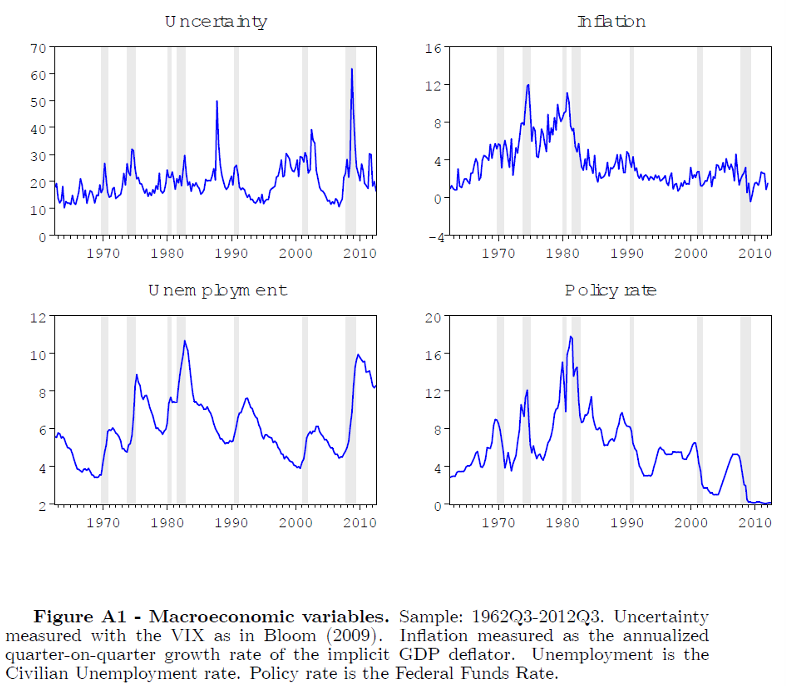
\includegraphics[width=0.75\linewidth]{macro var st var.png}
\end{figure}
\end{center}

\end{frame}



%======================================================
\begin{frame}{ST-VAR application}
%======================================================
\small

\textbf{Transition variable:}
\begin{itemize}
  \item $z_t$ is a \textbf{moving average of past GDP growth} (not unemployment)
  \item Low $z_t$ $\Rightarrow$ economy in (or near) \textbf{recession}.
  \item High $z_t$ $\Rightarrow$ economy in \textbf{expansion}.
\end{itemize}

\textbf{Logistic transition function} ($G \approx 0$ in expansions, $G \approx 1$ in recessions) = smooth \textbf{probability of being in recession}.

\medskip

\textbf{Calibration of $\gamma$:}
\begin{itemize}
  \item $\gamma$ is \textbf{calibrated} to $\gamma = 1.75$ (not estimated, since estimating it makes NLS extremely unstable):
  \item They choose $\gamma$ to \textbf{match the empirical frequency of recessions:}
\begin{itemize}
  \item $10\%$ recession probability $\;\Rightarrow\; \gamma = 2.4$
  \item $25\%$ recession probability $\;\Rightarrow\; \gamma = 1.2$
  \item mid-range $\;\Rightarrow\; \gamma = 1.75$ (their benchmark)
\end{itemize}
          \item $\gamma$ controls the \textbf{steepness} of transition.

\end{itemize}


\end{frame}


\begin{frame}{ST-VAR application: recession probability}
    \begin{figure}
        \centering
        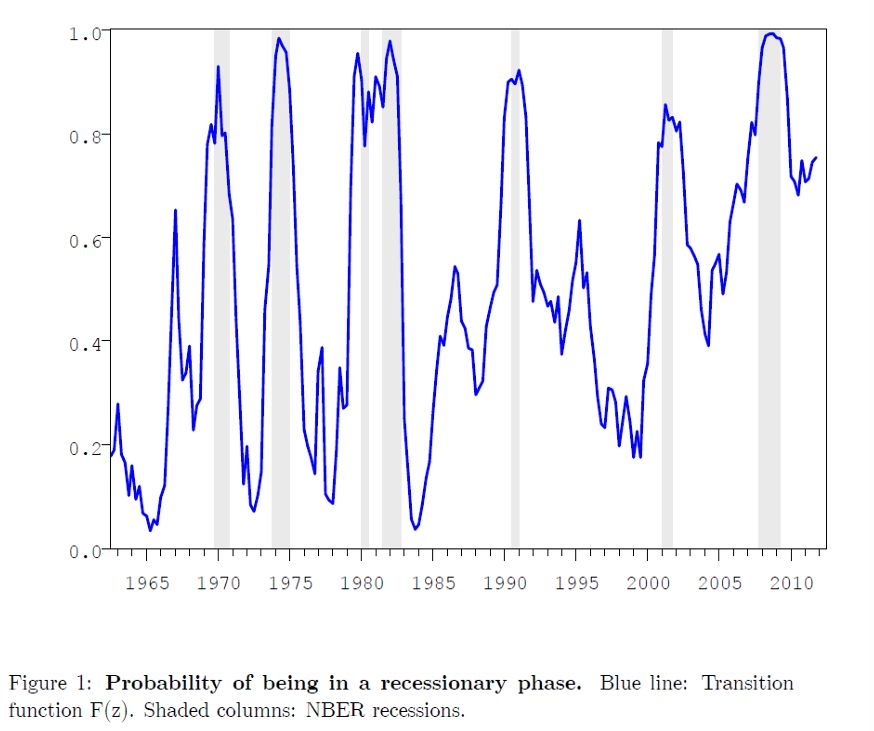
\includegraphics[width=1\linewidth]{proba of recession st var.png}
    \end{figure}
\end{frame}
%======================================================
\begin{frame}{ST-VAR application: IRF computation}
%======================================================
\footnotesize

\textbf{Two IRF scenarios:}
\begin{enumerate}
  \item \textbf{Expansion IRF:}
        start from a state where $G(z_t) \approx 0$ (good times).
  \item \textbf{Recession IRF:}
        start from a state where $G(z_t) \approx 1$ (bad times).
\end{enumerate}

\medskip

\textbf{Important assumption: Nonlinear IRFs must be computed under \textit{counterfactual} assumptions about the path of the state variable!}
\begin{itemize}
  \item As we have seen:
\begin{itemize}
\footnotesize
    \item a shock may push the economy toward recession or expansion,
    \item OR the shock may shift the transition variable itself,
    \item OR the regime may drift back to expansion after a few quarters,
    \item OR it may stay in recession for a long time.
    \end{itemize}
  \item So, after an uncertainty shock they assume the economy \textbf{stays in recession for 20 quarters} when simulating recession IRFs.
  \item long enough that \textbf{all IRFs die out} (their horizon is 20 quarters).
  \item $\Rightarrow$ keeps the regime \textbf{fixed} during the horizon, so that IRFs can be clearly interpreted as "recession" vs "expansion' responses.
  \item avoids contamination from an endogenous regime shift (the economy automatically leaving a recession due to the shock). 
\end{itemize}

\end{frame}



%======================================================
\begin{frame}{Results: linear IRFs to an uncertainty shock}
%======================================================
\footnotesize

\textbf{Linear VAR benchmark}: identify an \textbf{uncertainty shock} (e.g. Cholesky ordering with VIX first), compute IRFs of unemployment, inflation and FFR.

Gives the \textbf{average} effect of uncertainty shocks, pooling recessions and expansions.


\begin{center}
\begin{figure}
    \centering
    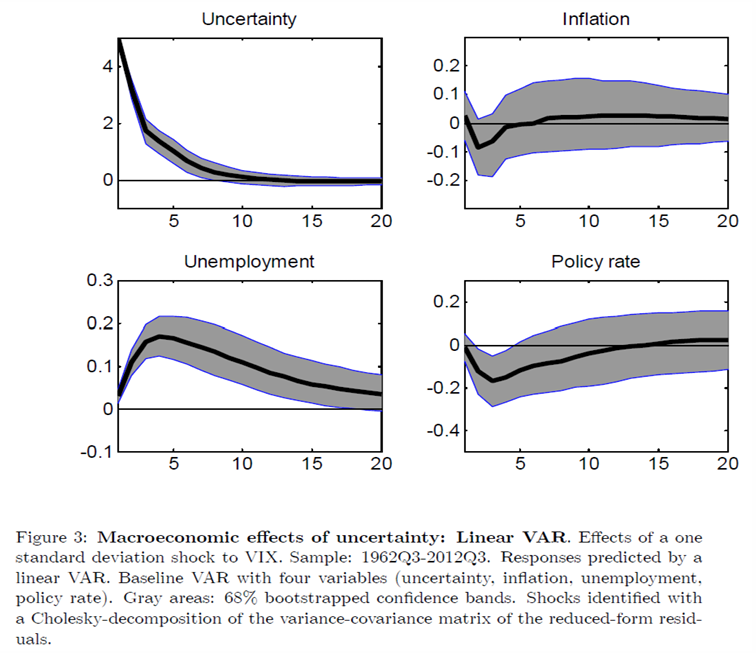
\includegraphics[width=0.7\linewidth]{IRF lin st var.png}
\end{figure}
\end{center}

\end{frame}
%======================================================
\begin{frame}{Results: nonlinear IRFs in recession vs expansion}
%======================================================
\footnotesize

\textbf{ST-VAR IRFs} starting from a \textbf{recession} state ( kept for 20 quarters).

\begin{itemize}
  \item Uncertainty shock: $\uparrow$ unemployment \textbf{much more} in recessions .
  \item Effects on inflation and the policy rate are also \textbf{strongly state-dependent}.
\textbf{  \item Linear VAR \textbf{understates} the importance of uncertainty
        during recessions.}
\end{itemize}

\begin{center}
\begin{figure}
    \centering
    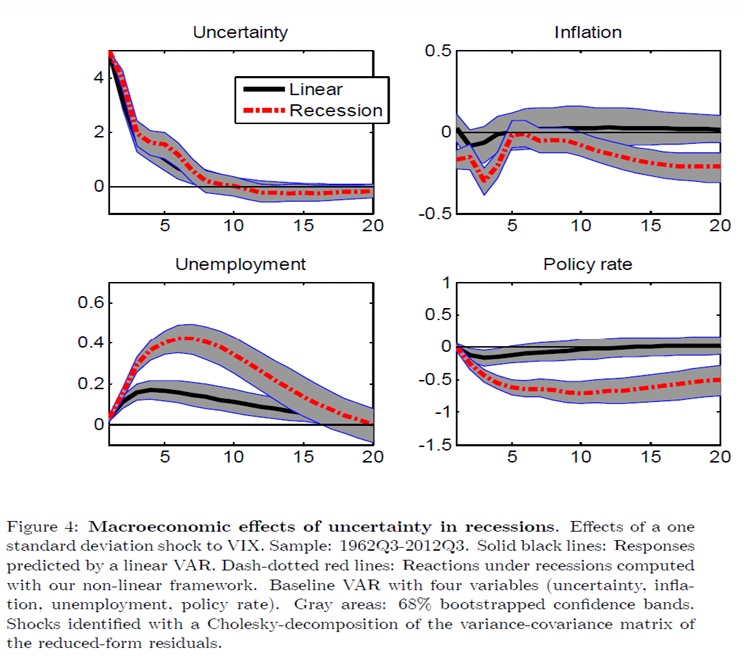
\includegraphics[width=0.6\linewidth]{IRF non lin st var.png}
\end{figure}
\end{center}

\end{frame}


%======================================================
\begin{frame}{Results: nonlinear IRFs in recession vs expansion on macro variables}
%======================================================

\begin{center}
\begin{figure}
    \centering
    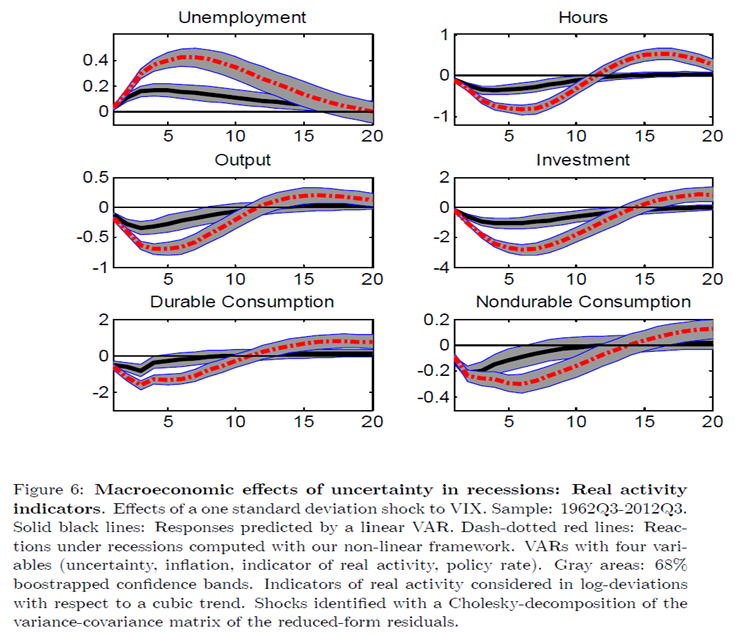
\includegraphics[width=0.8\linewidth]{IRF nonlin on macro var st var.png}
\end{figure}
\end{center}

\end{frame}


%======================================================
\begin{frame}{ST-VAR application: robustness}
%======================================================
\footnotesize

\textbf{Robustness:} They repeat the analysis with: alternative measures of uncertainty (e.g.\ other financial spreads, common factor of uncertainty indicators).

\medskip

\begin{center}
\begin{figure}
    \centering
    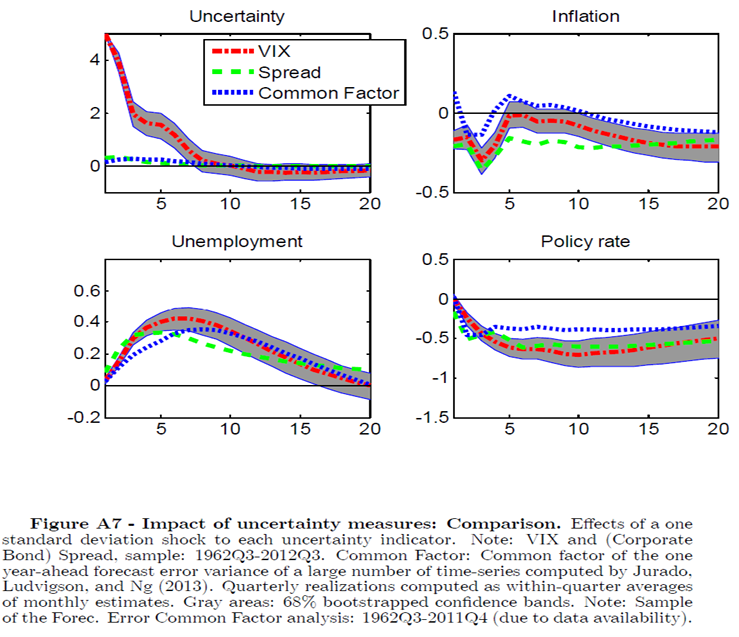
\includegraphics[width=0.7\linewidth]{robustness st var.png}
\end{figure}
\end{center}


\end{frame}




\section{Regime switching}


%======================================================
\begin{frame}{Markov regime switching}
%======================================================
\small
\begin{itemize}
    \item The covariance-stationary Markov-Switching (MS) model (Quandt, 1958; Neftçi, 1982, 1984;  Hamilton, 1989).
    \item Its success relies on its ability to reproduce the US business cycle instead of using a complex and non-transparent procedure (as implemented by the NBER Business Cycle Dating Committee, cf. Burns \& Mitchell (1946), \textit{Measuring Business Cycles}.
    \item In opposition to TAR models,\textbf{ the transition variable is not observed but is supposed to follow a first order Markov chain.}
\end{itemize}

\textbf{Goal:} allow the dynamics of $y_t$ to switch between a few \emph{regimes} (e.g.\ expansion vs recession),\textbf{ governed by a Markov chain.}

\begin{itemize}
  \item Regime switches are \textbf{discrete} (jumps) and\textbf{ governed by a probabilistic rule (the Markov chain).}
  \item Regimes are typically \textbf{latent}: \textbf{we do not directly observe $s_t$, but infer it from the data.}
\end{itemize}

\end{frame}

%======================================================
\begin{frame}{Markov-switching VAR (MS-VAR)}
%======================================================
\small

\textbf{Goal:} allow the dynamics of $y_t$ to switch between a few \emph{regimes} (e.g.\ expansion vs recession),\textbf{ governed by a Markov chain.}

\medskip
\textbf{MS-VAR($p$):}
\[
y_t = A_0^{(s_t)} + A_1^{(s_t)} y_{t-1} + \dots + A_p^{(s_t)} y_{t-p} + u_t,
\qquad u_t \sim \mathcal{N}\big(0,\Sigma^{(s_t)}\big)
\]
where:
\begin{itemize}
  \item $s_t \in \{1,\dots,K\}$: \textbf{regime index} at time $t$
        (e.g.\ $1=$ expansion, $2=$ recession).
  \item $A_j^{(i)}$, $\Sigma^{(i)}$: regime-specific coefficients and shock covariance matrices.
\end{itemize}

\textbf{Interpretation:}
\begin{itemize}
  \item Regime switches are \textbf{discrete} (jumps) and\textbf{ governed by a probabilistic rule (the Markov chain).}
  \item Regimes are typically \textbf{latent}: \textbf{we do not directly observe $s_t$, but infer it from the data.}
\end{itemize}

\end{frame}


%======================================================
\begin{frame}{What is a Markov chain (and why use it for regimes?)}
%======================================================
\footnotesize

A Markov chain is a random process that \textbf{moves between a finite number of states} (here: regimes), where\textbf{ the future depends only on the current state, not on the full past.}
\medskip

\textbf{Definition (informal):}
Let $s_t \in \{1,\dots,K\}$ denote the state at time $t$. Then $(s_t)$ is a \emph{Markov chain} if
\[
\Pr(s_t = j \mid s_{t-1}, s_{t-2},\dots)
= \Pr(s_t = j \mid s_{t-1}) \quad \forall j
\]

\begin{itemize}
  \item \textbf{"Memoryless"}: to forecast $s_t$, you only need to know $s_{t-1}$.
  \item Very natural for \textbf{phases} like:
        \begin{itemize}
        \footnotesize
          \item weather: \textit{sunny} / \textit{rainy},
          \item business cycle: \textit{expansion} / \textit{recession},
          \item financial markets: \textit{normal} / \textit{crisis}.
        \end{itemize}
\end{itemize}

\medskip

\textbf{But why is this useful for regime switching in macro?}
\begin{itemize}
  \item It gives a \textbf{probabilistic law} for entering and leaving regimes
        (no arbitrary dating rule / ad hoc threshold).
  \item It captures \textbf{persistence} (spells can be long) and \textbf{occasional jumps}.
  \item  And it is \textbf{parsimonious} (just a small set of transition probabilities!).
\end{itemize}

\end{frame}



%======================================================
\begin{frame}{The Markov chain for regimes (2-regime example)}
%======================================================
\small

\textbf{Assume two regimes:} $s_t \in \{1,2\}$. Each regime corresponds to a given phase of the economic cyle and for each date $t$, the economy can either stay in the same regime at date $t+1$ or switch to the other regime. 

\medskip
\textbf{Markov property:}
\[
\Pr(s_t = j \mid s_{t-1}=i, s_{t-2},\dots) =
\Pr(s_t = j \mid s_{t-1}=i) = p_{ij}
\]
\textbf{Transition matrix:}
\[
P =
\begin{bmatrix}
p_{11} & p_{12} \\
p_{21} & p_{22}
\end{bmatrix},
\qquad
p_{ij} = \Pr(s_t = j \mid s_{t-1} = i),
\quad
p_{i1} + p_{i2} = 1
\]
\pause
\begin{itemize}
  \item $p_{11}$: probability of staying in Regime 1 (e.g.\ expansion).
  \item $p_{22}$: probability of staying in Regime 2 (e.g.\ recession).
  \item $p_{12}$: probability of moving from Regime 1 to Regime 2.
  \item $p_{21}$: probability of moving from Regime 2 to Regime 1.
\end{itemize}


\end{frame}



%======================================================
\begin{frame}{The Markov chain for regimes (2-regime example)}
%======================================================
\small

\textbf{Expected duration of a regime:}
\[
\mathbb{E}[\text{length of Regime } i] = \frac{1}{1 - p_{ii}}
\]

\begin{itemize}
  \item If $p_{22}$ is close to 1, recessions are persistent.
  \item If $p_{11}$ is high, expansions last many periods on average.
  \item If $p_{12}$ is small: not about length but means that recessions are rare.
\end{itemize}

\pause
\textbf{Unconditional (long-run) probabilities:}

Imagine the regime indicator $s_t \in \{1,2\}$ evolves forever: even though at any date the regime is random, over very long horizons the \emph{empirical frequency} of being in each regime stabilizes. That limiting frequency is the \textbf{unconditional} or \textbf{stationary distribution}:
\[
\text{Fixed point: }\pi_{tomorrow} = \pi_{today} P, \quad \pi_1 + \pi_2 = 1
\]
gives the long-run fraction of time in each regime.

\end{frame}




%======================================================
\begin{frame}{MS-VAR: regime-dependent dynamics and IRFs}
%======================================================
\small

\textbf{Within each regime $i$:}
\[
y_t = A_0^{(i)} + A_1^{(i)} y_{t-1} + \dots + A_p^{(i)} y_{t-p} + u_t,
\qquad u_t \sim \mathcal{N}\big(0,\Sigma^{(i)}\big)
\]

Conditional on $s_t = i$ and \emph{staying} in regime $i$,
        we have an ordinary linear VAR with parameters $\{A_j^{(i)},\Sigma^{(i)}\}$

   \begin{itemize}
  \item \textbf{Expected IRF with switching:}
        \begin{itemize}
          \item account for the fact that future $s_{t+h}$ may switch according to $P$
          \item \textbf{the IRF becomes an expectation over all possible regime paths (given the state at the start of the IRF)}
        \end{itemize}
\end{itemize}

\begin{itemize}
  \item "Swiss-army knife"!
\end{itemize}

\end{frame}





%======================================================
\begin{frame}{Estimating an MS-VAR}
%======================================================
\footnotesize

\textbf{Key challenge:} the regime $s_t$ is \emph{latent}. It governs both the VAR coefficients and the shock variance,  
\textbf{but we never observe $s_t$ directly.}

\medskip

\textbf{Idea:} treat $s_t$ as hidden states of a Markov chain and use  \textbf{state-space filtering} to infer them.

\begin{enumerate}
    \item The issue of the \emph{observed} likelihood for the MLE is that it integrates out the unobserved $s_t$.
    \item \textbf{So Hamilton filter and smoothing = how we infer the regimes}
\begin{itemize}
\footnotesize
   \item \textbf{Forecasted prob.:}
\(\Pr(s_t=i \mid y_{1:t-1})\) - predicted regime before seeing $y_t$.
    \item  \textbf{Filtered prob. (forward recursion)} to update
\(\Pr(s_t=i \mid y_{1:t})\) - real-time estimate of the current regime.
    \item \textbf{Smoothed prob. (backward pass):}
\(\Pr(s_t=i \mid y_{1:T})\) - best ex-post estimate (uses full sample).
   \end{itemize}

    \item \textbf{Parameter estimation}: MLE + numerical optimisation
   \end{itemize}


\textbf{What we get:}
\begin{itemize}
\item Time series of \textbf{smoothed probabilities} of each regime, often interpreted as the \textbf{probability of recession}.
\item Regime-specific VAR parameter estimates and IRFs: how the transmission of shocks differs between regimes.
\end{itemize}

\end{frame}


%======================================================
\begin{frame}{MS-VAR example: Ferrara (2003)}
%======================================================
\small

\textbf{Reference:} Ferrara, L., A three-regime real-time indicator for the US economy (2003, \textit{Economics Letters})

\medskip
\textbf{Goal:} use an MS-VAR to \textbf{let the data themselves identify different phases of the US business cycle (no NBER dating imposed).}

\medskip
\textbf{Data:}
\begin{itemize}
  \item Monthly US data, \textbf{1985-2002}.
  \item 4 real-activity indicators: Industrial Production Index (IPI), Unemployment rate, Construction, Help-Wanted index.
        \end{itemize}

\medskip

\textbf{Model:} MS(3)-VAR(0)
\begin{itemize}
  \item 3 regimes, Markov chain $s_t \in \{1,2,3\}$.
  \item VAR(0): regime-dependent \textbf{means} (and possibly variances), but no lag dynamics:
        \[
          y_t = \mu^{(s_t)} + \varepsilon_t, 
          \qquad \varepsilon_t \sim \mathcal{N}(0,\Sigma^{(s_t)})
        \]
        \end{itemize}
 Each regime summarises a \textbf{different average level / volatility}
        of real activity (e.g.\ slump / normal / boom).


\end{frame}


%======================================================
\begin{frame}{MS-VAR example}
%======================================================


\textbf{Output of interest:}
\begin{itemize}
  \item Time series of \textbf{smoothed regime probabilities} (by MLE+Hamilton)
        \[
          \Pr(s_t = 1 \mid y_{1:T}),\;
          \Pr(s_t = 2 \mid y_{1:T}),\;
          \Pr(s_t = 3 \mid y_{1:T})
        \]
        \end{itemize}
These are interpreted as the probability that the economy is in
        each \textbf{latent business-cycle phase} at date $t$.


\medskip

\textbf{Empirical finding:}
\begin{itemize}
  \item The three regimes line up with \textbf{low / medium / high} activity phases and reproduce US business cycles without using NBER dates by construction!
  \item MS-VAR = an \textbf{automatic, model-based business-cycle dating tool}.
\end{itemize}


\end{frame}



\begin{frame}{Estimated probabilities of being in a regime for the US economy (Ferrara, 2003)}
    \begin{figure}
        \centering
        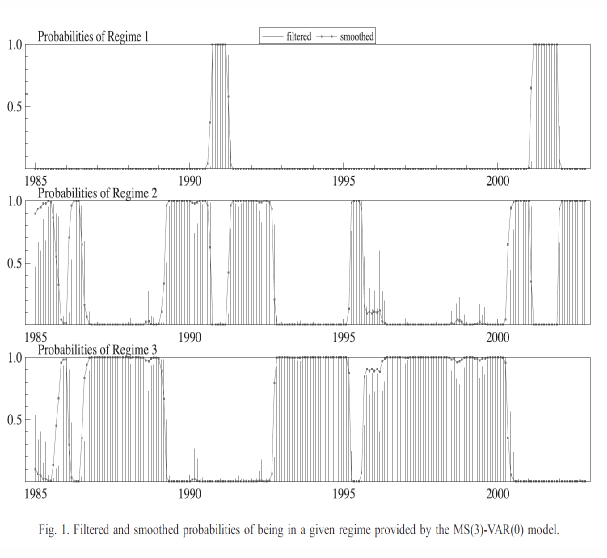
\includegraphics[width=0.75\linewidth]{proba recession Ferrara.png}
    \end{figure}
\end{frame}



\section{TVP}


\begin{frame}{Time-varying parameter VAR (TVP-VAR):}
    \textbf{Why should coefficients move?}
\begin{itemize}
  \item \textbf{E.g. inflation-output-rates block is not timeless:}
  \begin{itemize}
    \item Slope of the Phillips curve changes with bargaining power,
          globalization, unions' culture, job laws...
    \item Monetary policy reaction changes with Fed chairs (Volcker $\rightarrow$ Greenspan $\rightarrow$ Bernanke $\rightarrow$ Powell).
    \item Impact of interest rates on demand changes with leverage, financial
          frictions, demographics, etc.
  \end{itemize}
  \item These evolutions:
  \begin{itemize}
    \item do \emph{not} occur in only 2-3 regimes,
    \item do \emph{not} happen at a sharp threshold in one observable,
    \item but happen \textbf{gradually, continuously, and with uncertainty}.
  \end{itemize}
\end{itemize}

TVP-VAR: the \textbf{economic relationships themselves 
(the coefficients) \textbf{evolve over time, slowly and stochastically}.}

Seminar: Cogley \& Sargent (2001)
\end{frame}


%======================================================
\begin{frame}{Time-varying parameter VAR (TVP-VAR):}
%======================================================
\small

\textbf{From fixed to time-varying coefficients:}

\medskip
\textbf{Standard VAR($p$):} $A_j$ and $\Sigma$ are \textbf{constant} over time.

\textbf{TVP-VAR($p$):}
\[
y_t = A_{0,t} + A_{1,t} y_{t-1} + \dots + A_{p,t} y_{t-p} + u_t,
\qquad u_t \sim \mathcal{N}(0,\Sigma_t)
\]

\begin{itemize}
  \item $y_t$: $k \times 1$ vector of macro variables.
  \item $A_{j,t}$: $k \times k$ matrices of \textbf{time-varying coefficients}.
  \item $\Sigma_t$: \textbf{time-varying covariance matrix of reduced-form shocks.}
\end{itemize}

At each date $t$ we still have a \textbf{linear VAR}, but
\[
\{A_{j,t}, \Sigma_t\} \quad \text{are allowed to change over time}
\]

\begin{itemize}
  \item Captures gradual changes in behaviour, institutions, policy rules...
\end{itemize}

\end{frame}

%======================================================
\begin{frame}{TVP-VAR as a state-space model}
%======================================================
\scriptsize

\textbf{\textit{Measurement} (observation) \textit{equation}:}
\[
y_t = A_{0,t} + A_{1,t} y_{t-1} + \dots + A_{p,t} y_{t-p} + u_t,
\qquad u_t \sim \mathcal{N}(0,\Sigma_t)
\]

\textbf{State vector of parameters:}
\[
\theta_t =
\begin{bmatrix}
\mathrm{vec}(A_{0,t}) \\
\mathrm{vec}(A_{1,t}) \\
\vdots \\
\mathrm{vec}(A_{p,t}) \\
\mathrm{vech}(\Sigma_t)
\end{bmatrix}
\]

\textbf{\textit{State equation} (law of motion for parameters):}
\[
\theta_t = \theta_{t-1} + \eta_t,
\qquad \eta_t \sim \mathcal{N}(0,Q) \text{ with small variance}
\]
or more generally $\theta_t = F \theta_{t-1} + \eta_t$ with $F$ close to the identity matrix... So a \textbf{Random Walk!}

\begin{itemize}
  \item $\eta_t$ represents \textbf{parameter shocks} (slow structural drift).
  \item This is a \textbf{state-space model} (more on those in the next class):
        \begin{itemize}
        \footnotesize
          \item measurement equation: VAR with time-varying coefficients;
          \item state equation: evolution of coefficients and covariances.
        \end{itemize}
\end{itemize}

\begin{itemize}
  \item The macroeconomic structure is \textbf{not fixed} but evolves over time.
  \item TVP-VARs formalise this as a\textbf{ stochastic process for the parameters.}
\end{itemize}

\end{frame}


%======================================================
\begin{frame}{How can we \emph{estimate} a TVP-VAR if parameters follow a random walk?}
%======================================================
\footnotesize

The random-walk law for the parameters ($\theta_t$) is the \textbf{evolution constraint} that makes estimation possible. It is a \textbf{\textit{prior}}. 

\begin{itemize}
  \item At each date $t$, the coefficients $\theta_t$ are \textbf{latent states} (unobserved variables).
  \item The assumption $\theta_t = \theta_{t-1} + \eta_t$ (with \textbf{small variance})
        encodes the belief that macroeconomic relationships:
        \begin{itemize}\footnotesize
          \item evolve \emph{gradually}, not through abrupt jumps
          \item remain close to their past values unless data strongly indicates change.
        \end{itemize}
  \item The estimation problem becomes:
        \[
           \text{Find the smoothest path }\{\theta_t\}_{t=1}^T 
           \text{ that still explains the data } \{y_t\}_{t=1}^T 
        \]
   The computations of the \textbf{Kalman filter and smoother}!
\end{itemize}

\smallskip
\textbf{It belongs to State-Space models, models where:}  
\begin{itemize}
  \item The measurement equation says: "Given $\theta_t$, how likely is $y_t$?"
  \item The state equation says: "Given $\theta_{t-1}$, how plausible is $\theta_t$?"
  \item Estimation balances both:
        \begin{itemize}\footnotesize
          \item fit the data today (likelihood)
          \item  staying close to yesterday’s coefficients to avoid implausible jumps (random-walk prior).
        \end{itemize}
\end{itemize}

\end{frame}


%======================================================
\begin{frame}{What does a TVP-VAR buy us in practice?}
%======================================================
\small

\textbf{1. Time-varying dynamics and IRFs}

\begin{itemize}
  \item At each date $t$, given $\{A_{j,t}, \Sigma_t\}$, can compute usual VAR objects:
        \begin{itemize}

          \item \textbf{impulse responses conditional on specific time $t$, not on a "state" that can happen at diverse $t$! }
        \end{itemize}
  \item Let $\varepsilon_t$ be structural shocks with $u_t = C_t \varepsilon_t$, $C_t C_t' = \Sigma_t$.
\end{itemize}

\[
\text{IRF}_{h,t} =
\frac{\partial y_{t+h}}{\partial \varepsilon_t} \Big|_{\theta_t}
\quad \Rightarrow \quad
\text{IRF}_{h,t} \text{ depends on calendar time } t
\]

\begin{itemize}
  \item The response of output to a monetary policy shock in 1980
        can differ systematically from the response in 2010.
  \item Do not force one "average" IRF for the whole sample.
\end{itemize}

\textbf{2. Beyond discrete breaks}: time-located interpretation of parameters in a structural TVP-VAR.

\end{frame}

%======================================================
\begin{frame}{Estimation of TVP-VARs}
%======================================================
\small

TVP-VAR is a linear-Gaussian state-space model (more on those next class):
\[
\begin{cases}
y_t = Z_t(\theta_t) + u_t, & u_t \sim \mathcal{N}(0,\Sigma_t) \\
\theta_t = F \theta_{t-1} + \eta_t, & \eta_t \sim \mathcal{N}(0,Q)
\end{cases}
\]

\textbf{Estimation tools}
\begin{itemize}
  \item \textbf{Kalman filter (forward) and smoother (backward):}
        \begin{itemize}
          \item Filter: real-time updating. Recursively update beliefs about $\theta_t$ given data up to $t$
          \item Smoother: historical reconstruction of how the economy changed (obtaining estimates using full sample information $T$).
        \end{itemize}
  \item \textbf{Bayesian methods} are standard:
        \begin{itemize}
          \item place priors on $Q$, initial $\theta_0$ etc
          \item use MCMC / variational Bayes for posterior draws of
                $\{\theta_t\}_{t=1}^T$
          \item from each draw, compute time-varying IRFs.
        \end{itemize}
\end{itemize}


\end{frame}



\begin{frame}{Application: A time-varying finance-led Goodwin model}
%======================================================
\scriptsize

\textbf{Santetti (2024), "A time-varying finance-led model for U.S. business cycles"(Metroeconomica)} (following Carrillo-Maldonado \& Nikiforos, "Estimating a time-varying distribution-led regime" (Levy WP, 2022).

\begin{itemize}
\scriptsize
  \item \textbf{Goodwin pattern:} counter-clockwise cycles between employment and labour share.
  \item \textbf{Regimes:} profit-led demand \& profit-squeeze distribution; role of residential investment and finance.
\end{itemize}

\medskip
\textbf{TVP-VAR-SV model:} Endogenous vector $y_t = (\text{labour share},\ \text{employment rate},\ \text{residential investment},\ \text{term spread})'$ for US, quarterly, 1956-2019.
\begin{itemize}
  \item \textbf{TVP-VAR with stochastic volatility}
  \item Recursive (Cholesky) identification (finance $\rightarrow$ housing $\rightarrow$ employment $\rightarrow$ distribution): finance leads housing, housing leads the cycle, labour share reacts last.
  \item Bayesian estimation (Kalman filter in state-space form + Gibbs sampler).
\end{itemize}

\begin{itemize}
  \item Compute \textbf{time-varying IRFs} around six NBER peaks
        (1973Q1, 1981Q3, 1990Q3, 2001Q1, 2007Q4, 2019Q4).
  \item Track how demand and distributive regimes \textbf{change across business cycles}.
\end{itemize}

\medskip
\textbf{Main findings:} Evidence of \textbf{profit-led demand} and \textbf{profit-squeeze distribution} (Goodwin-type PL/PS regime).
\begin{itemize}
  \item Both regimes \textbf{weaken during the Great Moderation} then re-intensify pre-2019.
  \item \textbf{Residential investment} strongly \textbf{leads the cycle}.
  \item Results fit a \textbf{finance-led, deregulated} post-1980 US growth regime.
\end{itemize}

\end{frame}


\begin{frame}{}
\begin{figure}
    \centering
    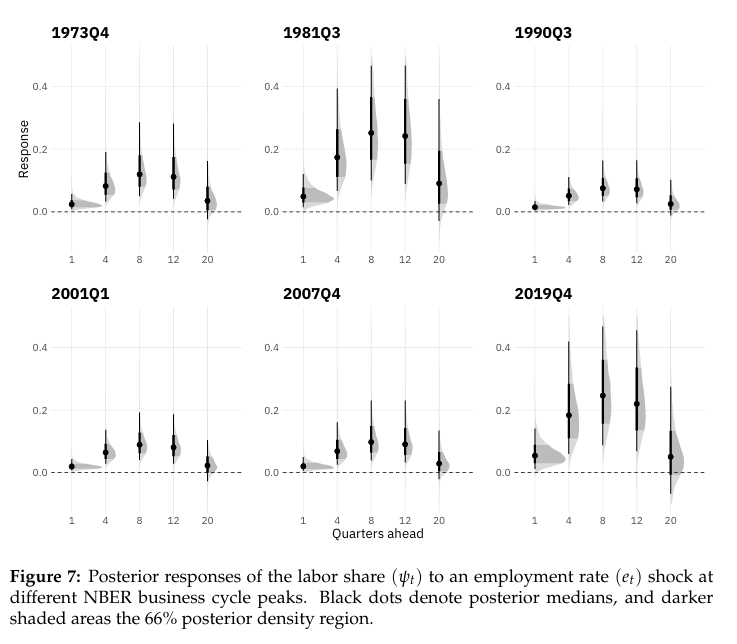
\includegraphics[width=0.9\linewidth]{irf goodwin tvp lab emp.png}
\end{figure}

\end{frame}

\begin{frame}{}
\begin{figure}
    \centering
    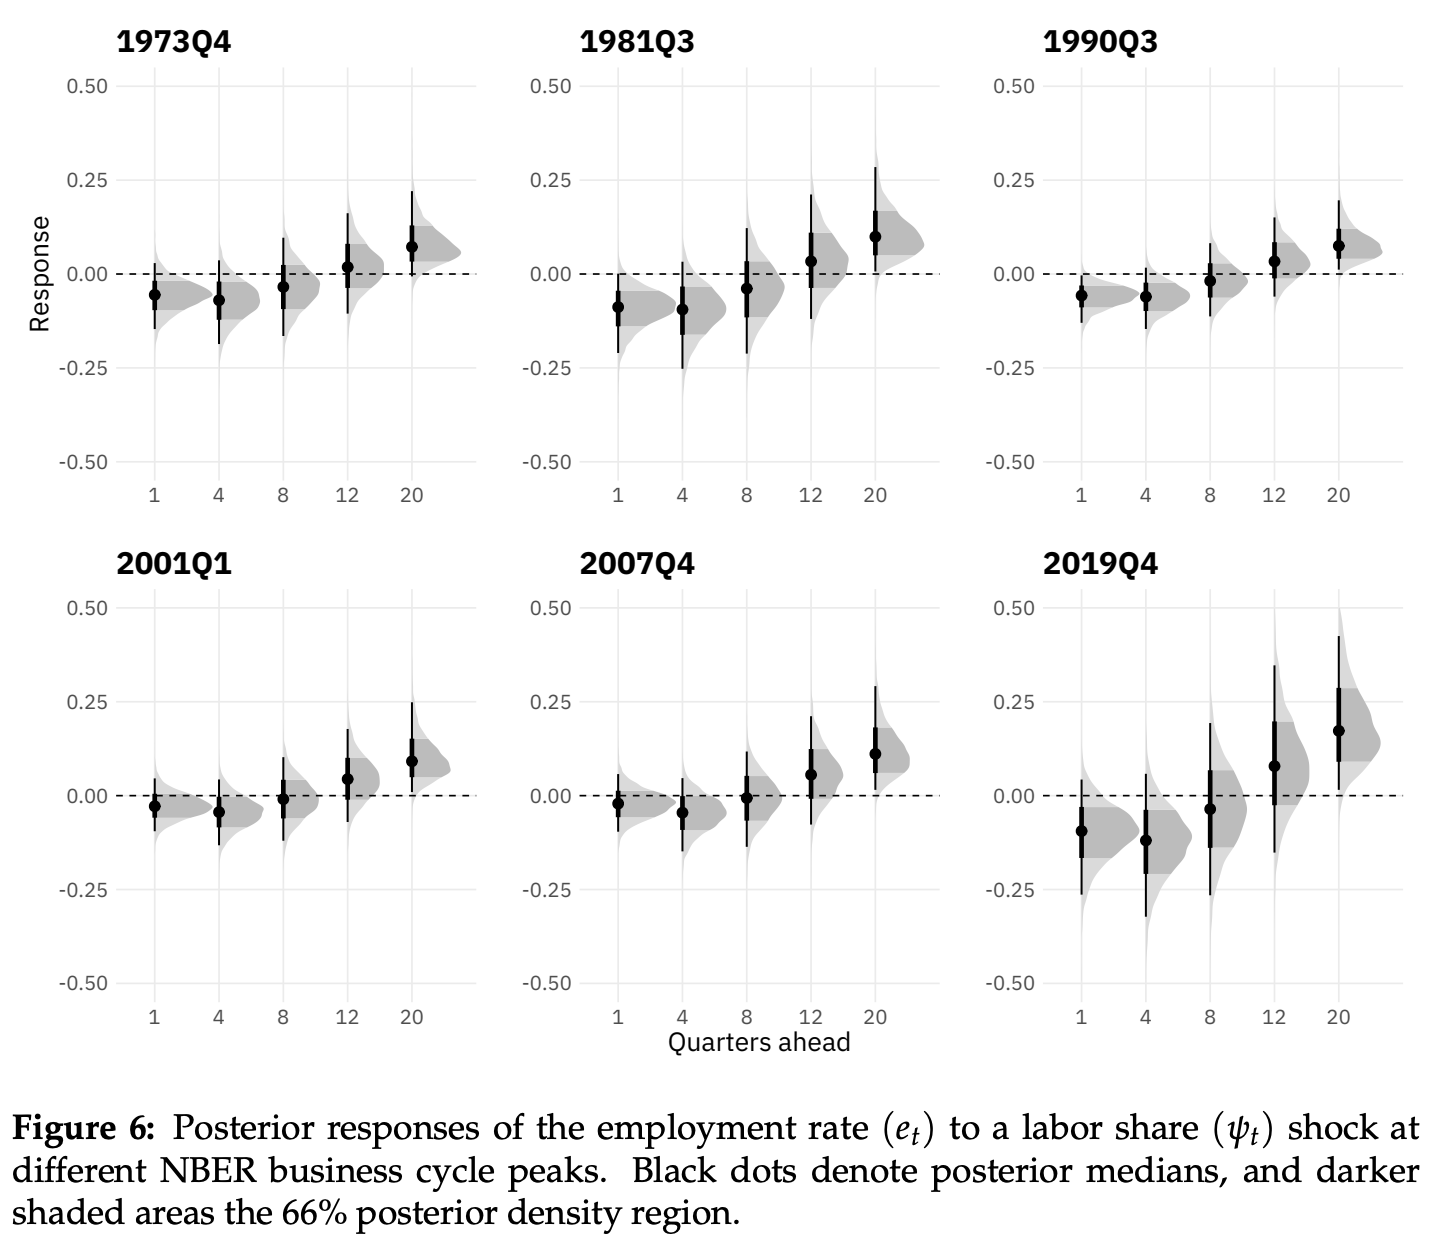
\includegraphics[width=0.9\linewidth]{TVP VAR Goodwin 1.png}
\end{figure}

\end{frame}


%======================================================
\begin{frame}{Recap}
%======================================================
\small
\textbf{TVAR / STVAR (Threshold / Smooth Transition VAR):}
  \begin{itemize}
    \item \emph{Use if} behaviour depends smoothly on an \textbf{observable variable} 
          (e.g.\ output gap, credit growth, interest rate level).
    \item Coefficients change \textbf{deterministically and abruptly (TVAR) / gradually as a mixture of states (STVAR)} with that variable (low vs high debt, low vs high inflation etc.).
  \end{itemize}

  \bigskip
  
\textbf{MS-VAR (Markov-switching VAR)}
  \begin{itemize}
    \item \emph{Use if} you suspect \textbf{unobserved discrete regimes} but \textbf{no clear observable variable} triggers transitions.
    \item Regime switches are \textbf{latent, probabilistic} (Markov chain), abrupt and \textbf{unobservable}.
  \end{itemize}

  \bigskip
\textbf{TVP-VAR (Time-Varying Parameter VAR):}
  \begin{itemize}
    \item \emph{Use if} you think the structure \textbf{drifts gradually over time} 
          (policy, expectations, institutions) \textbf{without clear regimes or triggers}.
    \item Coefficients follow a \textbf{stochastic drift} (often a random walk).
  \end{itemize}

\end{frame}






















%======================================================
\section{Local Projections}
%======================================================

%======================================================
\begin{frame}{From VAR-based IRFs to Local Projections}
%======================================================
\small

\begin{itemize}
  \item \textbf{So far:} We estimate a (S)VAR and recover (O)IRFs (either reduced form or structural/orthogonal). 
  \item The IRF at horizon $h$ is an \textbf{implied} object of the estimated VAR.
\end{itemize}

\pause

\begin{block}{Alternative: Local Projections (LPs)}
    
\textbf{Jordà, AER 2005}. See Jordà \& Taylor (JEL, 2025) for a state-of-the-art review.

\begin{itemize}
  \item Instead of deriving IRFs \emph{from} a VAR, we \emph{estimate} them
        \textbf{directly} by running separate regressions for each horizon $h$.
  \item For each horizon $h = 0,1,\dots,H$, estimate a regression of $y_{t+h}$
        on the shock at $t$ and suitable controls.
  \item The IRF at horizon $h$ is then just \textbf{a regression coefficient obtained by OLS
(one regression per horizon).}
\end{itemize}
\end{block}
\end{frame}


%======================================================
\begin{frame}{Baseline Local Projection with a known structural shock}
%======================================================
\footnotesize

 Let $\varepsilon_t$ be a \textbf{known structural shock} (e.g.\ a narrative series, temperature shocks).

\medskip
\textbf{Baseline LP:}
\[
y_{t+h} = \alpha_h + \beta_h \varepsilon_t + \Gamma_h X_{t-1} + u_{t+h},
\quad h = 0,1,\dots,H
\]

\begin{itemize}
  \item $y_{t+h}$: outcome $h$ periods after the shock.
  \item $\varepsilon_t$: identified structural shock at time $t$.
  \item $X_{t-1}$: vector of controls and lags (lags of $y_t$, lags of $\varepsilon_t$, and other covariates,
        time). Lags: either $p$ from VAR, or macro "rule" (4Q, 12M...).
  \item $\beta_h$: coefficient of interest:
        \[
          \beta_h \approx \frac{\partial y_{t+h}}{\partial \varepsilon_t}
        \]
        = \textbf{impulse response at horizon $h$}.
\end{itemize}

\textbf{Estimation:}
\begin{itemize}
  \item For each $h$, run a separate OLS regression.
  \item Collect $\{\hat{\beta}_h\}_{h=0}^H$ and plot them against $h$. Sequence $(\hat{\beta}_0,\dots,\hat{\beta}_H) =$ empirical IRF.
  \item Use HAC / Newey-West SEs to account for autocorrelation in $u_{t+h}$
        (which grows with $h$). And thus \textit{block }bootstrap for confidence bands.
        \end{itemize}
\end{frame}



%======================================================
\begin{frame}{Why Local Projections are useful}
%======================================================
\small

\begin{itemize}
  \item \textbf{Model-free IRFs:} no need to commit to a correct finite-order VAR.
  \item \textbf{More robust to misspecification} of the dynamic system (since no need for whole cross-correlation system, issue of lag number, omitted-variable bias due to dimensionality, wrong linearity...),
  \begin{itemize}
      \item  especially at longer horizons (since bad VAR iterates thus accumulate errors vs. LP as direct regression at $h+t$)
      \item LP \textbf{do not impose a dynamic system} since they only recover the local derivative of the conditional expectation at horizon \(h\) \(\beta_h = \operatorname{Cov}(y_{t+h}, \varepsilon_t)/\operatorname{Var}(\varepsilon_t)\)).  So linear projection is a consistent estimator.
  \end{itemize}
  \item \textbf{Flexibility:} easy to add
        \begin{itemize}
          \item nonlinear terms (interactions, thresholds, splines...): no need to estimate TVAR/STVAR.
          \item additional controls or instruments without over-dimensionality.
          \item constraints on $y_{t+h}$ (e.g.\ bounded outcomes: logit/probit).
        \end{itemize}
  \item $\Rightarrow$\textbf{Same toolbox as linear regression:} OLS, robust SE, IV, panel LPs, quantile LPs etc.
\end{itemize}
\end{frame}


%======================================================
\begin{frame}{Why Local Projections are useful}
%======================================================
\small

\textbf{Connection to VARs (Plagborg-Møller \& Wolf, 2021):}
\begin{itemize}
  \item If the true DGP is a linear VAR and $X_{t-1}$ contains enough lags,
        LPs and VAR-based IRFs estimate the \emph{same} population impulse responses.
  \item In finite samples there is a \textbf{bias-variance trade-off}:
        correctly specified VARs are more efficient,
        LPs are more bias-robust but can be noisier at long horizons.
\end{itemize}

\textbf{NB:} \textbf{VARs (especially Bayesian VARs) remain:}
\begin{enumerate}
    \item attractive when \textbf{precision at medium/long} horizons is crucial
    \item necessary when we have to\textbf{ build our exogenous shocks }by identification restrictions. \textbf{LP do not offer identification,} they need narrative/proxy series! (e.g. temperature shocks...)
\end{enumerate}

\textbf{NB:} \textbf{LP can be used for reduced-form analysis, identification is not necessary!} Cf. Jordà et al. papers "When Credit Bites Back" and "Leveraged Bubbles" (latter slide \textit{LPs in practice: credit booms, crises, and bubbles})!



\end{frame}



%======================================================
\begin{frame}{Example: Recessions vs Expansions with a known shock}
%======================================================
\small

Example of state-dependent IRFs via interacted LP (Auerbach \& Gorodnichenko, 2012): \textbf{assume the structural shock $m_t$ is known} (e.g.\ fiscal shock).

\medskip
\textbf{Business-cycle indicator:} $z_t = 1$ if NBER recession, $0$ if expansion.

\medskip
\textbf{Non-linear Local Projection (simple version without lags):}
\[
y_{t+h}
 = (\alpha_h^1 + \beta_h^1 m_t)\, z_t 
 + (\alpha_h^0 + \beta_h^0 m_t)\,(1 - z_t)
 + u_{t+h}
\]

\begin{itemize}
\item $\{\beta_h^1\}$ = IRFs to the shock \textbf{during recessions}.
\item $\{\beta_h^0\}$ = IRFs to the shock \textbf{during expansions}.

\end{itemize}

\medskip
(With lags: just add lags of $y_t$ and $m_t$ to the regression
(as in the general interacted LP above).

\end{frame}


%======================================================
\begin{frame}{Asymmetric effects: positive vs negative shocks}
%======================================================
\small

\textbf{Another question (beyond the "state-dependence" issue):} do \textbf{positive and negative shocks have \textbf{mirror} effects?}

\medskip
Let the structural shock be $Shock_t$. \textbf{Decompose into positive and negative parts:}
\[
Shock_t^+ =
\begin{cases}
Shock_t, & \text{if } Shock_t \ge 0,\\
0,       & \text{otherwise},
\end{cases}
\qquad
Shock_t^- = Shock_t - Shock_t^+
\]

\medskip
\textbf{Asymmetric Local Projections:}
\[
y_{t+h}
 = \alpha_h
 + \beta_h^+ Shock_t^+
 + \beta_h^- Shock_t^-
 + \Gamma_h X_{t-1}
 + u_{t+h}
\]

\begin{itemize}
  \item $\{\beta_h^+\}$: IRFs to \textbf{positive} shocks.
  \item $\{\beta_h^-\}$: IRFs to \textbf{negative} shocks.
\end{itemize}

\begin{itemize}
  \item NB: here $Shock_t^+$ and $Shock_t^-$ are \textbf{already identified} series,
        so we can treat them as exogenous regressors.
\end{itemize}

\end{frame}


\begin{frame}{Asymmetric IRFs to MP shocks}
    \begin{figure}
        \centering
        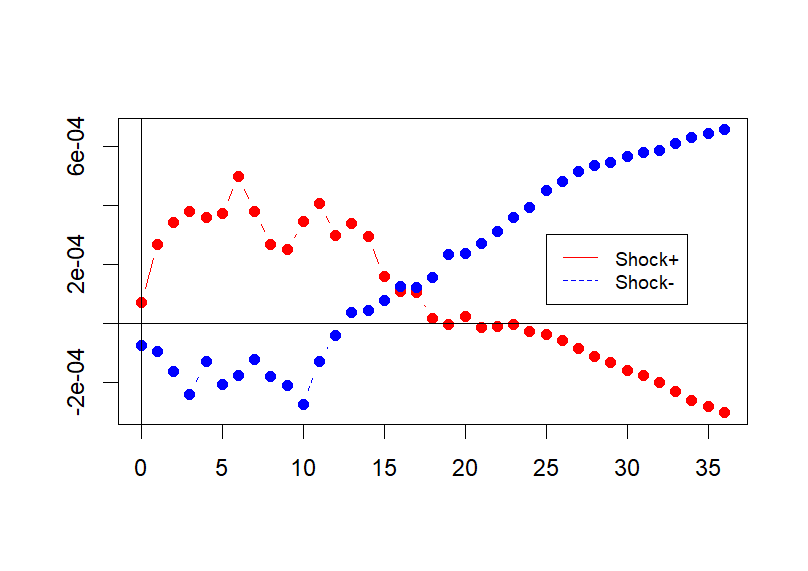
\includegraphics[width=1\linewidth]{Asym shock MP.png}
    \end{figure}
\end{frame}



%======================================================
\begin{frame}{LPs in practice: credit booms, crises, and bubbles}
%======================================================
\scriptsize

\textbf{1. Jordà, Schularick \& Taylor (2013) - \textit{When Credit Bites Back}}

\medskip


\textbf{Research question:} Do recessions become \textbf{deeper and longer} when they follow unusually fast \textbf{credit growth}? Are \textbf{financial-crisis} recessions systematically worse than normal ones?

\medskip

\textbf{How LPs are used (NO identified shock): } For every recession in a long-run panel (14 countries, 1870-2008), use LPs to trace the \textbf{recovery path of GDP} for 5 years after the pre-recession peak, conditional on \textbf{excess credit} before the downturn and \textbf{crisis vs non-crisis} episodes.

\medskip 
\textbf{Results:} Financial-crisis recessions are much more damaging: output remains far below trend even after 5 years. High pre-crisis credit growth predicts systematically \textbf{deeper and slower} recoveries (strong evidence of a \textbf{credit overhang} mechanism).

\bigskip

\textbf{2. Jordà, Schularick \& Taylor (2015) - \textit{Leveraged Bubbles}}

\medskip

\textbf{Research question:} Do \textbf{housing or equity bubbles} worsen the next recession? Are bubbles harmful only when they are \textbf{credit-fuelled}?

\medskip

\textbf{How LPs are used (NO identified shock)}
\begin{itemize}
  \item LPs compare medium-run GDP paths after recessions preceded by:
       (i) no bubble,  
        (ii) an "unleveraged" bubble,  
        (iii) a \textbf{credit-fuelled} (leveraged) bubble.
\end{itemize}

\medskip
\textbf{Results:} Equity bubbles modestly worsen recessions; housing bubbles are worse. But the real danger is \textbf{leverage}: credit-fuelled bubbles produce the \textbf{deepest and most persistent} output losses (often still negative after 5 years).
\end{frame}



%======================================================
\begin{frame}{LPs in practice: long-run effects of monetary policy}
%======================================================
\scriptsize

\textbf{3. Jordà, Schularick \& Taylor (2020) - \emph{The Long-Run Effects of Monetary Policy}}

\medskip
\textbf{Research questions:} Is monetary policy \textbf{neutral in the long run}, or do interest-rate
        shocks leave persistent scars on output, capital and TFP? Are long-run effects symmetric for \textbf{tightenings} vs \textbf{easings}?
        
\medskip
\textbf{How LPs are used}
\begin{itemize}
  \item Construct a long historical panel of advanced economies (20th century onward),
        with GDP, consumption, investment, capital and TFP.
  \item Use the \textbf{Mundell Trilemma} to build an external instrument for policy-rate
        changes (base-country rate shocks interacted with fixed FK regime and
        capital-openness).
  \item \textbf{IV LP}: for horizons up to 10-15 years, regress long-run changes in macro variables on the instrumented rate shock, with rich controls and country fixed effects; use robust panel standard errors.
  \item LP is chosen explicitly because it delivers \textbf{consistent long-horizon
        IRFs} when finite-lag VARs can be badly biased at long horizons.
\end{itemize}

\medskip
\textbf{Results:}
\begin{itemize}
  \item A one-percentage-point unexpected rate hike reduces real GDP by several
        percent even after a decade; capital and TFP show even stronger
        hysteresis, while hours largely recover.
  \item Tightening shocks have large and persistent real effects, but rate cuts do
        not symmetrically undo the damage (asymmetric hysteresis).
\end{itemize}

\end{frame}













\section{Homework}

%======================================================
\begin{frame}{Reading for next class: \textit{State-Dependent Fiscal Multipliers}}
%======================================================
\small

\textbf{Mandatory reading for next session}

\medskip
\begin{itemize}
  \item Fazzari, Morley \& Panovska (2015), \emph{“\href{https://www.degruyterbrill.com/document/doi/10.1515/snde-2014-0022/html?srsltid=AfmBOopPTA7blCwc6hBDY3TbsjhVfB8g7dNT6EnjONxQBHTvBh8fdJiD}{State-dependent effects of fiscal policy} ”},
        \textit{Studies in Nonlinear Dynamics \& Econometrics}.
  \item Why this paper?
    \begin{itemize}
      \item Go beyond the simple "recession vs expansion" (recessions are rare relative to expansions) or exceptions like the "ZLB", but look at\textbf{ economic slack vs. high capacity utilization, i.e. Keynesian idea of demand dynamics!}
      \item  Use a\textit{\textbf{ Bayesian}} \textbf{threshold SVAR}
      \item Solve investment puzzle of Blanchard-Perotti. 
    \end{itemize}
  \item Please read it carefully.
\end{itemize}

\end{frame}




\end{document}

